\documentclass[12pt, a4paper]{article}
\usepackage{url,graphicx,tabularx,array,geometry}
\usepackage[utf8]{inputenc}
\usepackage[ngerman]{babel}
\usepackage{paralist}
\usepackage{latexsym}
\usepackage{fancyhdr}
\usepackage{siunitx}
\usepackage{graphicx}
\usepackage{float}
\usepackage{color}

\pagestyle{fancy}

\usepackage{amsmath}
\usepackage{amsfonts}
\usepackage{amssymb}

\setlength{\parskip}{1ex} %--skip lines between paragraphs
\setlength{\parindent}{0pt} %--don't indent paragraphs

%-- Commands for header
\newcommand{\headerline}{\begin{tabularx}{\textwidth}{X>{\raggedleft}X}\hline\\\end{tabularx}\\[-0.5cm]}
\newcommand{\headerleftright}[2]{\begin{tabularx}{\textwidth}{X>{\raggedleft}X}#1%
& #2\\\end{tabularx}\\[-0.5cm]}
%\linespread{2} %-- Uncomment for Double Space

\usepackage{listings}
\usepackage{color}

\definecolor{dkgreen}{rgb}{0,0.6,0}
\definecolor{gray}{rgb}{0.5,0.5,0.5}
\definecolor{mauve}{rgb}{0.58,0,0.82}

\lstset{frame=tb,
  language=Java,
  aboveskip=3mm,
  belowskip=3mm,
  showstringspaces=false,
  columns=flexible,
  basicstyle={\small\ttfamily},
  numbers=none,
  numberstyle=\tiny\color{gray},
  keywordstyle=\color{blue},
  commentstyle=\color{dkgreen},
  stringstyle=\color{mauve},
  breaklines=true,
  breakatwhitespace=true
  tabsize=3
}



\begin{document}
\renewcommand{\headrulewidth}{0pt}
\fancyhf{}
\fancyhead[L]{
\headerleftright{\textbf{Turáns Graphtheorem}}{Daniel Schmidt}}
\fancyfoot[C]{\thepage}

\title{Turáns Graphtheorem}
\date{\today}
\author{Daniel Schmidt\\ Betreuer: Peter Munstermann}

\maketitle\thispagestyle{empty}

\begin{abstract}
Diese Ausarbeitung entstand im Rahmen des Seminars Kombinatorik im Wintersemester 2013/2014 und behandelt drei Beweise des Satz von Turáns.
\end{abstract}
\newpage

\section{Einleitung}
\label{theorem:einleitung}
Diese Ausarbeitung beschäftigt sich mit Turáns Graphtheorem, auch Satz von Turán genannt. Dieser ist in der extremalen Graphentheorie einzuordnen und gibt eine obere Schranke für die maximale Anzahl an Kanten in einem p - cliquenfreien Graphen an.\\
Im Folgenden werde ich zunächst Definitionen für die in den Beweisen verwendeten Begriffe liefern und danach werde ich die drei Beweisen vorstellen, welche den Kern dieser Ausarbeitung bilden. \\
Zunächst wird das Theorem über eine vollständige Induktion bewiesen, die sich die Struktur der Turán Graphen zu eigen macht. \\
In dem zweiten vorgestellten Beweis werden wir das Theorem über eine Gewichtsverteilung beweisen. \\
Der letzte Beweis bedient sich der Annahme, der gegebene Graph sei maximal und zeigt schließlich, dass dieser ein Turán Graph sein muss. Dieser erreicht wie sich im folgenden zeigen wird unter gewissen Umständen für die Kantenanzahl die obere Schranke welche im Theorem gegeben ist.

\section{Definitionen}
\subsection{Anmerkungen}
Es sei gesagt, dass die Konstante vor sämtlichen Graphen (r - Turán Graph, p - Clique, etc) Element der natürlichen Zahlen ist.

\subsection{Ungerichteter Graph}
\label{theorem:ungerichteter-graph}
Der ungerichtete Graph G = (V,E) sei definiert als Knotenmenge V
\begin{gather}
\begin{split}V = \{ v_1, ..., v_n \}\end{split}\notag\\\begin{split}\end{split}\notag
\end{gather}
und Kantenmenge E, wobei zwei Knoten $v_i, v_j$ benachbart heißen, falls
\begin{gather}
\begin{split}\{v_i, v_j\} \in E\end{split}\notag\\\begin{split}\end{split}\notag
\end{gather}

\subsection{Grad eines Knotens}
\label{theorem:grad-eines-knotens}
Der Grad $d_m$ eines Knotens $v_m$ ist definiert als die Anzahl der benachbarten Knoten, sprich
\begin{gather}
\begin{split}d_m = \text{  } \mid \{ v_i \mid v_i \in V \wedge \{ v_i, v_m \} \in E \} \mid\end{split}\notag\\\begin{split}\end{split}\notag
\end{gather}

\subsection{Vollständiger Graph}
Ein Graph G = (V,E) heißt vollständig, falls alle Knoten durch Kanten verbunden sind. Es gilt also 

\begin{align*}
	E  = \{ \{ v_i , v_j \} \mid v_i, v_j \in V  \wedge v_i \neq v_j \}
\end{align*}

\subsection{Untergraph von G}
Ein Graph G' = (V', E') heißt Untergraph von G = (V, E), falls $V' \subseteq V$ und $E' \subseteq E$ gilt. 

\subsection{p - Clique im Graph G}
\label{theorem:p-clique-im-graph-g}
Ein Graph heißt p - Clique im Graph G, falls er ein vollständiger Untergraph von G mit p Knoten ist.


\subsection{Unabhängige Knotenmenge}
\label{theorem:unabhangige-knotenmenge}
Eine Menge von Knoten wird als unabhängig bezeichnet, wenn es innerhalb dieser Menge keine Kanten gibt, sondern nur nach Knoten außerhalb dieser.


\subsection{r - partiter Graph}
\label{theorem:r-partiter-graph}
Ein r - partiter Graph besteht aus $r \in \mathbb{N}$  disjunkten und unabhängigen Knotenmengen, welche untereinander durch Kanten verbunden sein können. Diese Knotenmengen bilden zudem eine Partition der gesamten Knotenmenge.


\subsection{Vollständiger r - partiter Graph}
\label{theorem:vollstandiger-r-partiter-graph}
Ein r - partiter Graph wird vollständig genannt, wenn jeder Knoten mit jedem anderen verbunden ist, außer mit denen, die in einer unabhängigen Knotenmenge mit ihm sind.


\subsection{r - Turán Graph}
\label{theorem:turan-graph}
Ein r - Turán Graph ist ein vollständiger r - partiter Graph bei dem sich die Größe jeder Partition maximal um 1 unterscheidet.


\subsection{Turáns Graphtheorem}
Sei $p \in \mathbb{N} \wedge p \ge 2$,  G = (V, E) ein Graph ohne p - Clique und n := $\mid V \mid$, so gilt
\begin{align} 
\mid E \mid \le (1- \frac{1}{p-1}) \frac{n^2}{2}
\end{align}



\section{Beweis über strukturelle Induktion}
\label{proof/second:zweiter-beweis-struktur-des-turan-graphs}\label{proof/second::doc}
In diesem Beweis nutzen wir die Struktur eines Turán Graphens aus und beweisen im Folgenden die stärkere Forderung ''Sei G ein Graph ohne p - Clique, dann besitzt G höchstens so viele Kanten wie der (p - 1) - Turán Graph". \\
Aus dieser Behauptung folgt direkt der Satz von Turán, denn ein kantenmaximaler, p - cliqenfreier Graph G=(V,E) mit $\mid V \mid = n$ muss aufgrund der Forderung ein Turán Graph sein. \\
Dieser hat genau dann die meisten Kanten, wenn alle Partitionen gleich groß sind, was der Fall ist, wenn n durch (p - 1) teilbar ist, es also $\frac{n}{p-1}$ Partitionen gibt. Daraus folgt für die Anzahl der Kanten:
\begin{gather}
\begin{split}&\text{Anzahl der Verbindungsmöglichkeiten zwischen je (p - 1) Knoten} \\
&\cdot ( \text{Anzahl der unabh. Teilmenge} )^2 = \\ &{ p - 1 \choose 2 } ( \frac{n}{p-1} )^2 = (1 - \frac{1}{p - 1}) \frac{n^2}{2}\end{split}\notag\\\begin{split}\end{split}\notag
\end{gather}
und unsere Behauptung ist bewiesen. Nun folgt der Beweis der stärkeren Forderung:


\subsection{Sei G ein Graph ohne p - Clique, dann besitzt G höchstens so viele Kanten wie der (p - 1) - Turán Graph}
\label{proof/second:sei-g-ein-graph-ohne-p-clique-dann-besitzt-g-hochstens-so-viele-kanten-wie-der-p-1-turan-graph}
\subsubsection{Induktionsanfang:}

Beginnen wir mit p = 2, so kann ein Graph G keine Kanten besitzen, da ein 2 - Clique aus einer Kante besteht. Ebendies gilt auch für einen 1 - Turán Graph, dieser besteht aus einer unabhängigen Teilmenge, hat also ebenfalls keine Kanten. 

\subsubsection{Induktionvoraussetzung:}

Sei G ein Graph ohne p - Clique. Dann besitzt G höchstens so viele Kanten wie der (p - 1) - Turán Graph.

\subsubsection{Induktionsschluss:}

Sei ein (p + 1)-cliquenfreier Graph G gegeben mit der Knotenmenge V und einer Kantenmenge E. Nun setzen wir $v_m$ so, dass für dessen Grad gilt $d_m := max_{1 \le j \le n} d_j$, sprich wir suchen uns einen Knoten mit den meisten Kanten im Graphen aus.

Nun setzen wir S als Menge der Nachbarn von $v_m$, wodurch $\mid S \mid = d_m$ ist und definieren $T := V \backslash S$. Da alle Knoten aus S mit $v_m$ verbunden sind, $v_m \notin S$ und G (p + 1)-cliquenfrei ist, muss S p-cliquenfrei sein.

Definieren wir nun H als neuen Graphen mit identischer Knotenmenge, für den nur die Kanten aus S übernommen werden und jeder Knoten aus S mit jedem aus T verbunden ist. Da in T keine Kanten übernommen werden, ist T eine unabhängige Menge in H und damit (p + 1)-cliquenfrei.

\begin{figure}[H] 
		\centering
		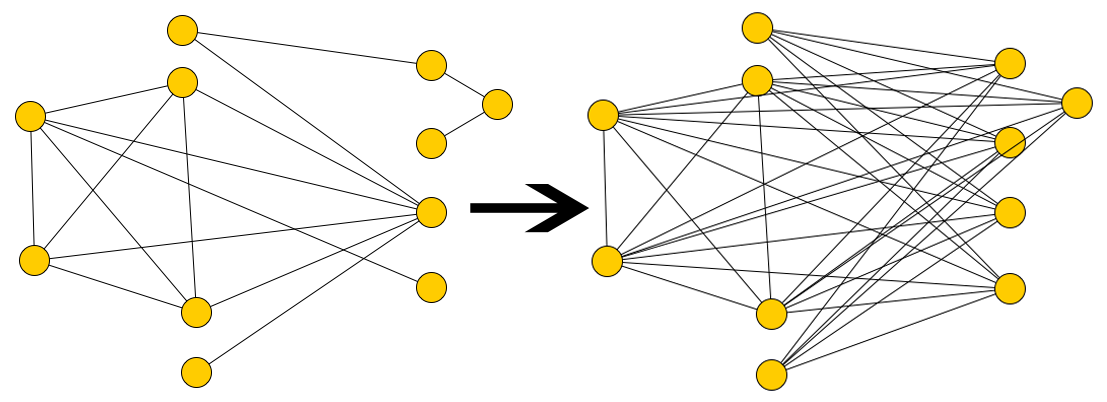
\includegraphics[page=1, width=\textwidth]{assets/proof2}
		\caption{Konstruktion von H} 
\end{figure}

Bezeichnen wir den Grad eines Knotens $v_j$ in H als $d'_j$. Untersucht man nun die Grade in H, so lassen sich zwei Fälle unterscheiden:

\textbf{Fall 1:} $v_j \in S$

Hier gilt $d'_j \ge d_j$, da keine Kanten entfernt wurden, aber eventuell welche hinzugefügt wurden.

\textbf{Fall 2:} $v_j \in T$

Es gilt $d'_j =^1 \mid S \mid = d_m \ge^2 d_j$.
\begin{enumerate}
\item {}
gilt, da jedes Element aus T mit jedem Element aus S eine Kante teilt.

\item {}
gilt, da $v_m$ so gewählt wurde, dass $d_m$ maximal ist.

\end{enumerate}

Hieraus folgt $\forall v_j \in V: d'_j \ge d_j$ und somit auch $\mid E(H) \mid \ge \mid E \mid$.

Da S wie gezeigt p-cliquenfrei ist, lässt sich hier die Induktionsvoraussetzung anwenden, sprich S kann maximal so viele Kanten haben wie ein (p - 1) - Turán Graph haben. Dementsprechend lässt sich H' als neuer Graph konstruieren, bei dem S ein (p - 1) - Turán Graph ist und wie beim Graphen H jeder Knoten aus T mit jedem aus S verbunden ist. Durch diese Konstruktion ist H' auf jeden Fall ein p - partiter Graph und hat dadurch höchstens so viele Kanten wie ein p-Turán Graph, wodurch unsere Behauptung bewiesen ist.


\section{Beweis über Gewichtsverteilung}
\label{proof/third::doc}\label{proof/third:dritter-beweis-gewichtsverteilung}
In diesem Beweis betrachten wir eine Gewichtsverteilung auf den Knoten des Graphen. Diese notieren wir als $w = (w_1,...,w_n)$ und es gilt $w_i \ge 0$, sowie $\sum^n_{i=1}w_i = 1$. Des weiteren definieren wir eine Funktion $f(w) = \sum_{ \{v_i, v_j\} \in E} w_i w_j$, welche wir zu maximieren versuchen. Wir nutzen diese Funktion, da sie für den ganzen Graphen dann maximal ist, wenn die Gewichte möglichst gleichmäßig verteilt sind.

Setzen wir nun $v_i$ und $v_j$ als zwei nicht benachbarte Knoten mit positivem Gewicht $w_i, w_j$ und fassen das Gewicht ihrer adjazenten Knoten zusammen als $s_i, s_j$ und nehmen $s_i \ge s_j$ an.

\begin{figure}[H] 
		\centering
		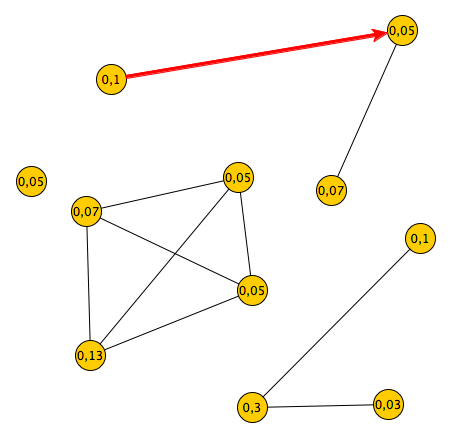
\includegraphics[page=1, width=\textwidth]{assets/proof3_first_move}
		\caption{Gewichtsverschiebung zwischen nicht benachbarten Knoten} 
\end{figure}

Bewegen wir nun das Gewicht von $v_j$ nach $v_i$, setzen also $w'_i := w_i + w_j$ und $w'_j := 0$, dann ergibt sich für die neue Gewichtung $w'$:
\begin{gather}
\begin{split}f(w') &=^1 f(w) + w_j s_i - w_j s_j \\
&= f(w) + (s_i - s_j) w_j \\
&\ge^2 f(w)\end{split}\notag\\\begin{split}\end{split}\notag
\end{gather}\begin{enumerate}
\item {}
Dies gilt aufgrund des verschobenen Gewichts. Dieses wird in der Multiplikation auf seitens $s_j$ nicht mehr betrachtet, bei $s_i$ schon. Da $w_j$ für $s_j$ wegfällt, wird das Gewicht hier also abgezogen und bei $s_i$ umgekehrt hinzugerechnet in der Multiplikation.

\item {}
Dies gilt, da $(s_i - s_j) w_j \ge 0$ ist.

\end{enumerate}

Wir können diese Verschiebung nun wiederholen bis es keine nicht-adjazenten Knoten mit positiver Gewichtung mehr gibt und erhalten danach eine optimierte Verteilung, da für jede Umformung $f(w') \ge f(w)$ gilt. Da wir das Gewicht nach einer bestimmten Anzahl an Verschiebungen in eine k - Clique verschoben haben, betrachten wir nun wie wir das Gewicht für eine solche Clique optimieren können. \\
Das Gewicht muss in einer k-Clique sein, da bei jeder Verschiebung mindestens ein Knoten aus der Menge der Knoten herausfällt, die verschoben werden können. Daher muss sich das Gewicht so lange Sammeln, bis es keine nicht benachbarten Knoten mit positiven Gewicht mehr gibt. \\
Die sich bildende Clique muss nicht zwangsweise die größte Clique sein, aber f wäre dann am Ende größer als mit einer kleineren Clique.

\begin{figure}[H] 
		\centering
		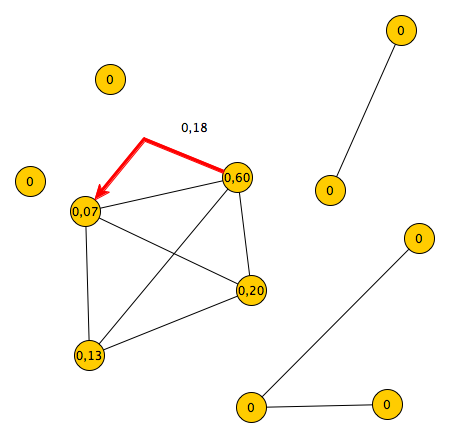
\includegraphics[page=1, width=\textwidth]{assets/proof3_before_first_moving_step}
		\caption{Gewichtsverschiebung innerhalb der Clique} 
\end{figure}

Bewegen wir die Gewichte innerhalb einer solchen k - Clique in der Form, dass wir uns zwei Knoten mit positiven Gewicht wählen für die $w_i > w_j > 0$ gilt und ein $\varepsilon$ setzen für das $0 < \varepsilon < w_i - w_j$ gilt. Addieren wir $\varepsilon$ auf $w_j$ und subtrahieren es von $w_i$. Es ergibt sich also:
\begin{gather}
\begin{split}f(w') &=^1 f(w) - w_i w_j + w'_i w'_j \\
&= f(w) - w_i w_j + (w_i - \varepsilon)(w_j + \varepsilon) \\
&= f(w) + \varepsilon (w_i - w_j) - \varepsilon^2 \\
&>^2 f(w)\end{split}\notag\\\begin{split}\end{split}\notag
\end{gather}\begin{enumerate}
\item {}
Dies gilt, da in einer Clique alle Knoten miteinander verbunden sind, gleichen sich die Unterschiede für die Funktionswerte für alle Kanten aus, außer der zwischen $v_i$ und $v_j$. Dementsprechend muss das alte Gewicht abgezogen und das neue addiert werden.

\item {}
Dies gilt, da $0 < \varepsilon < w_1 - w_2$ gilt.

\end{enumerate}

Daher optimiert diese Gewichtsverlagerung die k-Clique bis es keine ungleichen Gewichtungen mehr in ihr gibt.
Dass dies irgendwann eintritt, ist leicht einzusehen, denn wenn man $\varepsilon$ setzt als
\begin{gather}
\begin{split}\varepsilon := w_i - \frac{1}{k}\end{split}\notag\\\begin{split}\end{split}\notag
\end{gather}
wodurch $w_i' = w_i - \varepsilon = w_i - w_i + \frac{1}{k} = \frac{1}{k}$ gilt, also ein Knoten nach dem anderen die optimale, da gleichmäßige Verteilung einnimmt, wodurch sich die Anzahl der Knoten mit unterschiedlichem Gewicht schrittweise verringert. Hierzu muss $0 < w_i - \frac{1}{k} < w_i - w_j$, also $w_j < \frac{1}{k} < w_i$ gelten. Wenn man $w_i$ als maximal gewichteten Knoten wählt und $w_j$ als minimal gewichteten, dann muss $\frac{1}{k}$ zwischen beiden liegen. Obrige Ungleichung hat gezeigt, dass je näher die Werte der einzelnen Knoten aneinanderliegen, desto optimierter ist die Funktion f, wodurch bei einer gleichmäßigen Verteilung das Optimum liegt. Dies liegt an der Eigenschaft der Multiplikation maximal für die Summe der Faktoren zu sein, wenn beide Faktoren gleich groß sind.

\begin{figure}[H] 
		\centering
		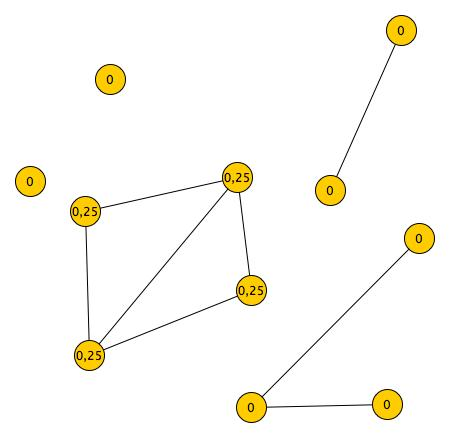
\includegraphics[page=1, width=\textwidth]{assets/proof3_after_second_moving_step}
		\caption{uniforme Gewichtsverteilung innerhalb der Clique} 
\end{figure}

In einer k-Clique können sind genau $\frac{k (k-1)}{2}$ Kanten, also \\
 $\frac{\text{Jeder Punkt} (\text{Jeder Punkt mit dem er sich verbinden kann})}{\text{Enden einer Kante}}$. Für die Gewichtung ergibt sich also:
\begin{gather}
\begin{split}f(w) &=^1 \sum_{v_i, v_j \in E} w_i w_j =^2 \sum_{v_i, v_j \in E} \frac{1}{k^2}  \\
&= \mid E \mid \frac{1}{k^2} =^3 \frac{k (k-1)}{2} \frac{1}{k^2}  \\
&= \frac{k (k-1)}{2k^2} = \frac{k-1}{2k} = \frac{1}{2} (1 - \frac{1}{k})\end{split}\notag\\\begin{split}\end{split}\notag
\end{gather}\begin{enumerate}
\item {}
Definition von f.

\item {}
Setzung von $w_i := \frac{1}{k}$.

\item {}
Dies gilt, da wie oben erwähnt in einer k-Clique genau $\frac{k (k-1)}{2}$ Kanten sind.

\end{enumerate}

Da diese Funktion maximal ist wenn k maximal ist und der höchstmögliche Wert für k genau p - 1 ist, gilt weiter:
\begin{gather}
\begin{split}f(w) &= \frac{1}{2} (1 - \frac{1}{k}) \\
&\le \frac{1}{2} (1 - \frac{1}{p-1})\end{split}\notag\\\begin{split}\end{split}\notag
\end{gather}
Insbesondere gilt dies dann auch für die uniforme Verteilung
\begin{gather}
\begin{split}&\frac{\mid E \mid}{n^2} = f(w_i = \frac{1}{n}) \le \frac{1}{2} (1 - \frac{1}{p-1}) \\
\Longleftrightarrow &\mid E \mid = f(w_i = \frac{1}{n})  n^2 \le \frac{1}{2} (1 - \frac{1}{p-1})  n^2\end{split}\notag\\\begin{split}\end{split}\notag
\end{gather}

Dies ist die im Satz von Turán als obere Schranke angegebene Kantenanzahl, wodurch dieser bewiesen ist.

\section{Beweis über den maximaler Graph und eine Äquivalenzrelation}
\label{proof/fifth:funfter-beweis-maximaler-graph-und-aquivalenzrelation}\label{proof/fifth::doc}\label{proof/fifth:index-1}
In diesem Beweis wird angenommen, dass G=(V,E) ein Graph mit n Knoten und ohne p - Clique ist, welcher unter diesen Eigenschaften die maximale Anzahl an Kanten hat.
Um $\mid E \mid \le (1- \frac{1}{p-1}) \frac{n^2}{2}$ zu zeigen bedient sich dieser Beweis zudem folgender Behauptung:

\textbf{Behauptung:} G enthält keine drei Knoten u,v,w mit $\{ v, w \} \in E$, aber $\{ u, v \} \notin E$ und $\{ u, w \} \notin E$

Diese Behauptung beweisen wir durch Widerspruch. Hierzu unterteilen wir das Problem in zwei Fälle:

\begin{figure}[H] 
		\centering
		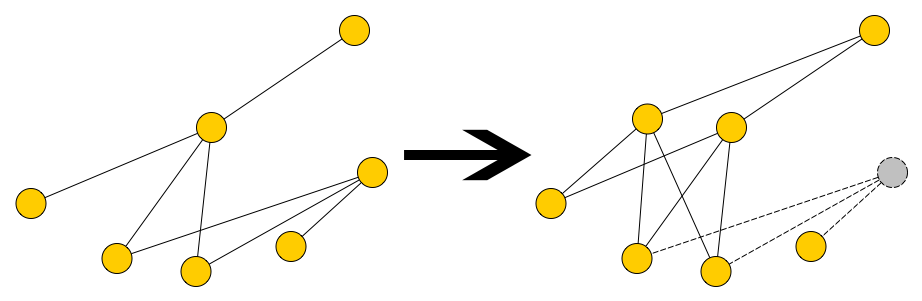
\includegraphics[page=1, width=\textwidth]{assets/proof5-case1}
		\caption{1. Fall} 
\end{figure}

\textbf{Fall 1:} $d(u) < d(v) \vee d(u) < d(w)$

Nehmen wir an, dass d(u) \textless{} d(v) gilt, denn u und v sind austauschbar.
Entfernen wir nun u, verdoppeln wir v und nennen den neuen Knoten v', wobei alle Kanten ebenfalls kopiert werden, sodass v' die selben Nachbarn wie v hat. Der hieraus entstehende Graph G' hat ebenfalls keine p-Clique, da v' bestehende Cliquen nicht erweitern kann, denn v und v' sind nicht verbunden. Hieraus ergibt sich für die Kantenanzahl:
\begin{gather}
\begin{split}\mid E(G') \mid = \mid E(G) \mid + d(v) - d(u) \overset{\text{da } d(u) < d(v)}{>} \mid E(G) \mid\end{split}\notag\\\begin{split}\end{split}\notag
\end{gather}
Da G ein maximaler Graph ist, ist dies ein Widerspruch.


\begin{figure}[H] 
		\centering
		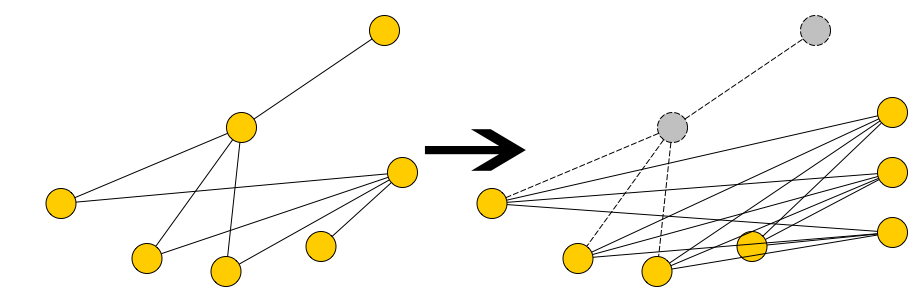
\includegraphics[page=1, width=\textwidth]{assets/proof5-case2}
		\caption{2. Fall} 
\end{figure}

\textbf{Fall 2:} $d(u) \ge d(v) \wedge d(u) \ge d(w)$

Hier kopieren wir u zwei mal, da es vom Grad her unter den drei Knoten maximal ist, wobei wie im ersten Fall die Kanten mitkopiert werden. Danach entfernen wir dann v und w. Der hieraus entstehende Graph kann wieder keine p-Clique haben, da die Kopien von u untereinander nicht verbunden sind. Für die Anzahl der Kanten ergibt sich:
\begin{gather}
\begin{split}\mid E(G') \mid &= \mid E(G) \mid + 2 d(u) - (d(v) + d(w) - 1) \\
&> \mid E(G) \mid\end{split}\notag\\\begin{split}\end{split}\notag
\end{gather}
Hierbei ergeben sich die $2d(u)$ durch das doppelte Kopieren von u, die $- (d(v) + d(w) - 1)$ vom Entfernen von v und w, sowie der Kante vw. Die Ungleichung gilt, da $d(u) \ge d(v) \wedge d(u) \ge d(w)$ gilt. Da G' nun mehr Kanten hat als G, ergibt sich wieder ein Widerspruch, womit die Behauptung bewiesen wäre.

Definieren wir $u \sim v :\Longleftrightarrow \{ u,v \} \notin E(G)$, so ist dies dank der bewiesenen Behauptung eine Äquivalenzrelation:

\textbf{Reflexivität:}
\begin{gather}
\begin{split}u \sim u \Longleftrightarrow^1 \{ u,u \} \notin E(G)\end{split}\notag\\\begin{split}\end{split}\notag
\end{gather}\begin{enumerate}
\item {}
Dies gilt, da die hier betrachteten Graphen keine Kanten mit gleichem Start und Zielknoten erlauben.

\end{enumerate}

\textbf{Transitivität:}
\begin{gather}
\begin{split} v \sim u \wedge u \sim w \Longrightarrow^1 v \sim w\end{split}\notag\\\begin{split}\end{split}\notag
\end{gather}\begin{enumerate}
\item {}
Dies ist exakt die oben bewiesene Behauptung.

\end{enumerate}

\textbf{Symmetrie:}
\begin{gather}
\begin{split}u \sim v &\Rightarrow \{ u,v \} \notin E(G) \\
&\Rightarrow\ v \sim u\end{split}\notag\\\begin{split}\end{split}\notag
\end{gather}

Für den Graphen G bilden die Äquivalenzklassen bezüglich $\sim$ die verschiedenen Partitionen, wodurch G ein r - partiter Graph ist. Da er p - cliquenfrei und maximal ist muss er aus p - 1 Partitionen bestehen, daher ist G ein vollständiger (p - 1) - partiter Graph. Würde G aus weniger Partitionen bestehen ließen sich durch Aufteilung zweier Partitionen mehr Kanten hinzufügen, was die Kantenmaximalität verletzen würde. Das bedeutet, wenn wir zeigen können, dass ein (p - 1) - Turán Graph mindestens so viele Kanten besitzt wie ein vollständiger (p - 1) - partiter Graph, dann folgt daraus, dass die Anzahl der Kanten von G genau wie in Beweis zwei ableitbar sind, sprich Turáns Graphtheorem gilt.

\subsection{Ein r - Turán Graph hat immer mindestens so viele Kanten wie ein beliebiger  r - patiter Graph}
Dass ein r-patiter Graph höchstens so viele Kanten wie ein vollständiger r-partiter Graph hat, wird als trivial vorausgesetzt. Zudem seien bei einem r - partiten Graphen $K_{n_1,...,n_r}$  die Partitionen gegeben als $V_1, ..., V_r$. \\
Es ist zu zeigen, dass die Anzahl der Kanten in einem vollständigen r - partiten Graphen $K_{n_1,...,n_r}$ genau dann maximal ist, wenn $\mid n_i - n_j \mid \le 1$ f.a. i,j $\in \{1, ...,  r \}$ gilt.

Wir nehmen für unseren r-partiten Graphen an, dass $\mid n_i - n_j \mid > 1$, also gilt ohne Beschränkung der Allgemeinheit $n_1 \ge n_2 + 2$ gilt.
Verschieben wir einen Knoten aus $V_1$ in die Partition $V_2$, so erhalten wir einen Graphen $K_{n_1 - 1, n_2 + 1,...,n_{p - 1}}$. Dieser besitzt aufgrund der Verschiebung $(n_1 - 1)(n_2 + 1) - n_1 n_2$ mehr Knoten als der ursprüngliche Graph, denn es gilt
\begin{gather}
\begin{split}(n_1 - 1)(n_2 + 1) - n_1 n_2 &= n_1 n_2 - n_2 + n_1 - 1 - n_1 n_2 \\
&= n_1 - n_2 - 1 \\
&\ge^1 n_2 + 2 - n_2 - 1 \\
&= 1\end{split}\notag\\\begin{split}\end{split}\notag
\end{gather}\begin{enumerate}
\item {}
Dies gilt, da $n_1 \ge n_2 + 2$ vorausgesetzt wird.

\end{enumerate}

Daher hat ein Turán Graph mindestens so viele Kanten wie ein entsprechender r - patiter Graph, wodurch Turáns Graphtheorem gilt.
\end{document}